% !TeX spellcheck = en_US
%\documentclass[11pt,a4paper]{article}
\documentclass[11pt
  , a4paper
  , article
  , oneside
%  , twoside
%  , draft
]{memoir}

\usepackage{control}
\usepackage[numbers]{natbib}


\begin{document}

\newcommand{\technumber}{
  RAON Control-Document Series\\
  Revision : v1.0,   Release : 2015-03-03 fixed date}
\title{\textbf{Timing System 개발환경 구성}}

\author{이상일\thanks{silee7103@ibs.re.kr} \\

  Rare Isotope Science Project\\
  Institute for Basic Science, Daejeon, South Korea
}
\date{\today}

\renewcommand{\maketitlehooka}{\begin{flushright}\textsf{\technumber}\end{flushright}}
%\renewcommand{\maketitlehookb}{\centering\textsf{\subtitle}}
%\renewcommand{\maketitlehookc}{C}
%\renewcommand{\maketitlehookd}{D}

\maketitle

\begin{abstract}
RAON accelerator는 대형 실험 장치로 많은 실험 장치들과 부대시설 장치로 구성되어 운영된다. 이러한 많은 실험 장치들을 제어하기 위한 제어 시스템들은 넓은 범위로 분산되어 구성되어 있으며 이러한 분산 환경에서의 많은 제어시스템들을 전체의 하나의 제어시스템으로 운영하기 위하여 RAON control system은 정밀한 타임 동기화가 필요하다. RAON 제어시스템은 정밀한 타이밍 동기화를 위하여 EVG/EVR 시스템을 사용한다. 본 문서는 EPICS와 연동되어 사용 되는 EVG/EVR Timing 시스템 개발 및 운영을 위한 환경 구성에 대하여 설명한다.
\end{abstract}

RAON accelerator에서 사용되는 Timing System은 Micro-Research Finland Oy 사의 EVG(Event Gengerator)/EVR(Event Receiver) 시스템을 사용한다. EVG/EVR Timing System은 많은 대형장치에서 사용되고 있는 검증된 Timing System 이다. EVG/EVR Timing System에 대한 특징은 아래와 같다.

\begin{itemize}
	\item Event driven system, 255 event codes
	\item 외부 RF reference clock을 이용한 event 신호 생성
	\item 50 ~ 125MHz Event clock rate
	\item Events generated
	\begin{itemize}
			\item From external HW inputs
			\item Two sequencers (up to 2048 events/sequencer)
			\item Multi counters
	\end{itemize}
	\item Cascaded Event Generators
	\item Different Clock Synchronization
\end{itemize}

EVG/EVR Timing System은 크게 VME 또는 cPCI interface 상에서 동작하며, RAON에서는 VME interface 상에서 운영되는 플랫폼 구조를 채택하였다. Timing System을 구성하는 항목은 크게 아래와 같다.

\begin{itemize}
	\item Hardware 구성 항목
	\begin{itemize}
		\item GPS 수신 장치
		\item SRS Clock source
		\item EVG/EVR/Fanout 보드
		\item MVME 6100/MVME 3100 보드 
		\item VME form factor		
	\end{itemize}
	\item Software 구성항목
	\begin{itemize}
		\item Workbench 3.3, vxWorks 개발 툴
		\item vxWorks 6.9 Realtime Operating System
		\item RTEMS Realtime Operating System
		\item MRFIOC2  
		\item EPICS		
	\end{itemize}
\end{itemize}

상위에 언급된 Hardware 구성은 BNC 및 SMA connector등으로 연결된다. Hardware 구성에 대한 내용은 다음 장에서 상세하게 다룬다. 소프트웨어 구성은 EVG/EVR에 대한 Event code 설정 등에 대한 interface 및 제어를 위하여 MRF2IOC가 개발되어 사용된다. 이는 실시간 환경구성을 위하여 MVME6100 및 MVME3100 보드 상에서 vxWorks 또는 RTEMS라는 실시간 운영체제 상에서 구동 된다.

\chapter{Hardware 구성}
각 로컬 제어시스템들이 Timing System으로 부터 Event 신호를 받기 위한 전체 구성에 대한 흐름도 및 
Timing System의 개발 및 운영에 필요한 Hardware 구성을 설명한다.
\clearpage

\section{전체 구성도}
\begin{figure}[h!]
	\centering
	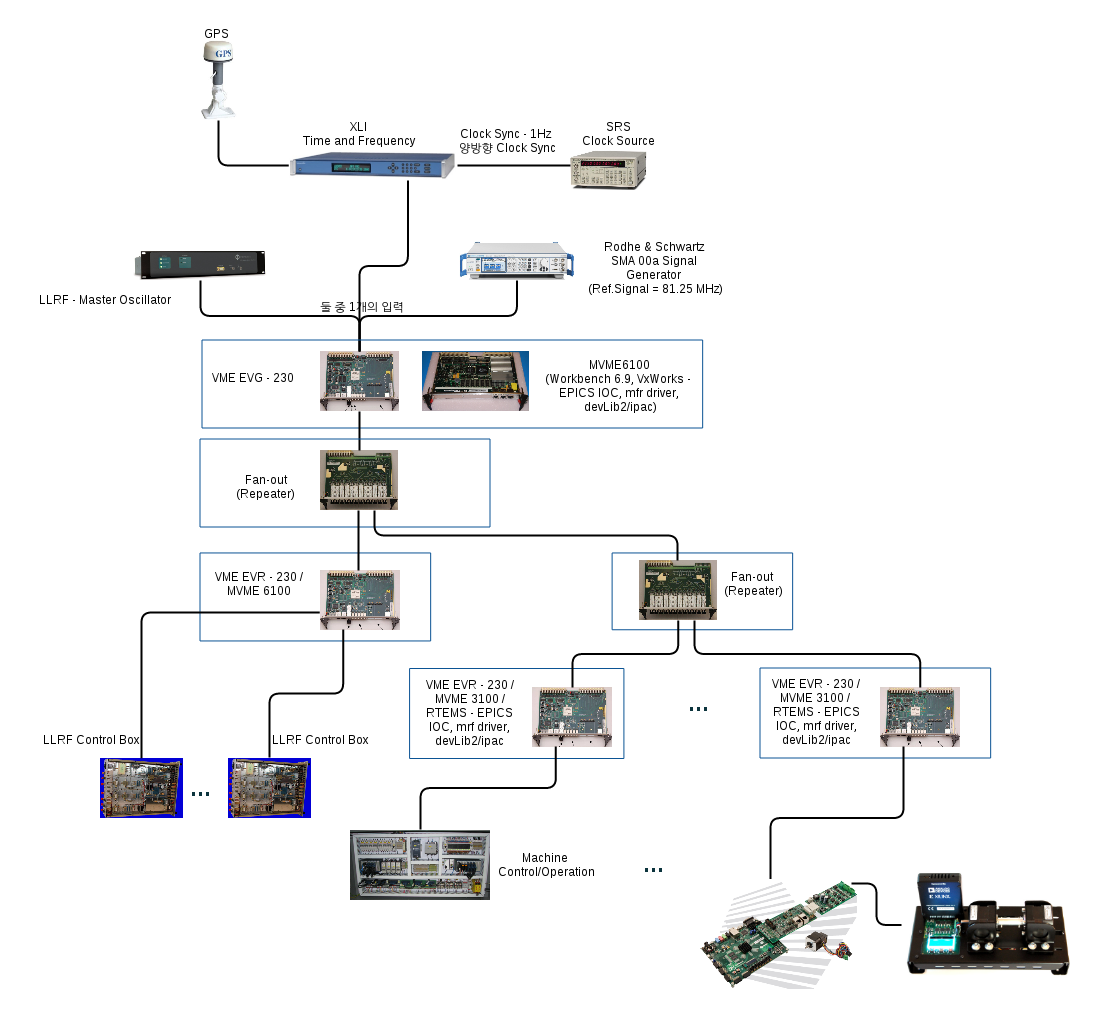
\includegraphics[width=1.1\textwidth, height=1.2\textwidth]{./images/timing_conf.eps}
	\caption{Timing System 전체 구성 흐름도}
	\label{fig:timing_conf} 
\end{figure}
 그림 \ref{fig:timing_conf}에서와 같이 RAON 가속기에서 사용될 Timing System에 대한 전체적인 구성 흐름을 볼 수 있다. 구성의 흐름을 살펴 보면, GPS로 부터 시각정보를 입력받아 Clock Source로 부터 1Hz로 Clock이 동기화 된다. 이 시각 정보는 Event Generator의 입력신호로 입력된다. 또한 EVG는 외부 RF Clock 신호를 입력으로 받아 Event Signal를 생성해 낼 수 있다. RAON 가속기기의 Reference Clock은 LLRF의 Master Oscillator로 부터 81.25MHz의 clock을 사용한다. Timing System의 개발 및 운영을 위하여 개발기간 동안은 LLRF의 Master Clock 대신 임시로 Signal Generator를 이용하여 81.25MHz의 Clock을 사용한다. EVG는 GPS 및 RF Clock 신호를 입력받아 Event를 생성하여 EVR에게 광모듈을 통하여 전달한다. EVG의 신호를 여러 장치로 전달하기 위하여 EVG와 EVR 사이에 Fanout 모듈이 사용 될 수 있다. Fanout 모듈은 Signal Repeater로 불리기도 하며 EVG 신호를 분배하는 역할을 수행한다. EVR은 EVG 또는 Fanout 모듈로 부터 광통신 모듈을 통하여 Event Signal을 획득하며, 최종적으로는 TTL 및 CML 형태의 신호를 로컬 제어장치에게 보낸다. 로컬 제어장치는 정밀하게 동기화된 Event Signal을 받아서 정의된 Event Code에 따라 로컬 제어로직을 수행한다. 
 
\section{EVG, Event Generator}
EVG는 Event Signal를 생성하는 Timing System에서 중추적인 보드이다. 동기화된 Timing Clock과 Timestamp를 제공하기 위하여 GPS 신호를 입력신호로 받는다. 그림 \ref{fig:evg_230_board}과 그림\ref{fig:evg_230_front}은 VME-based EVG-230 보드에 대한 그림과 front panel에 대한 port 구성도를 보여준다.

\begin{figure}[h!]
	\centering
	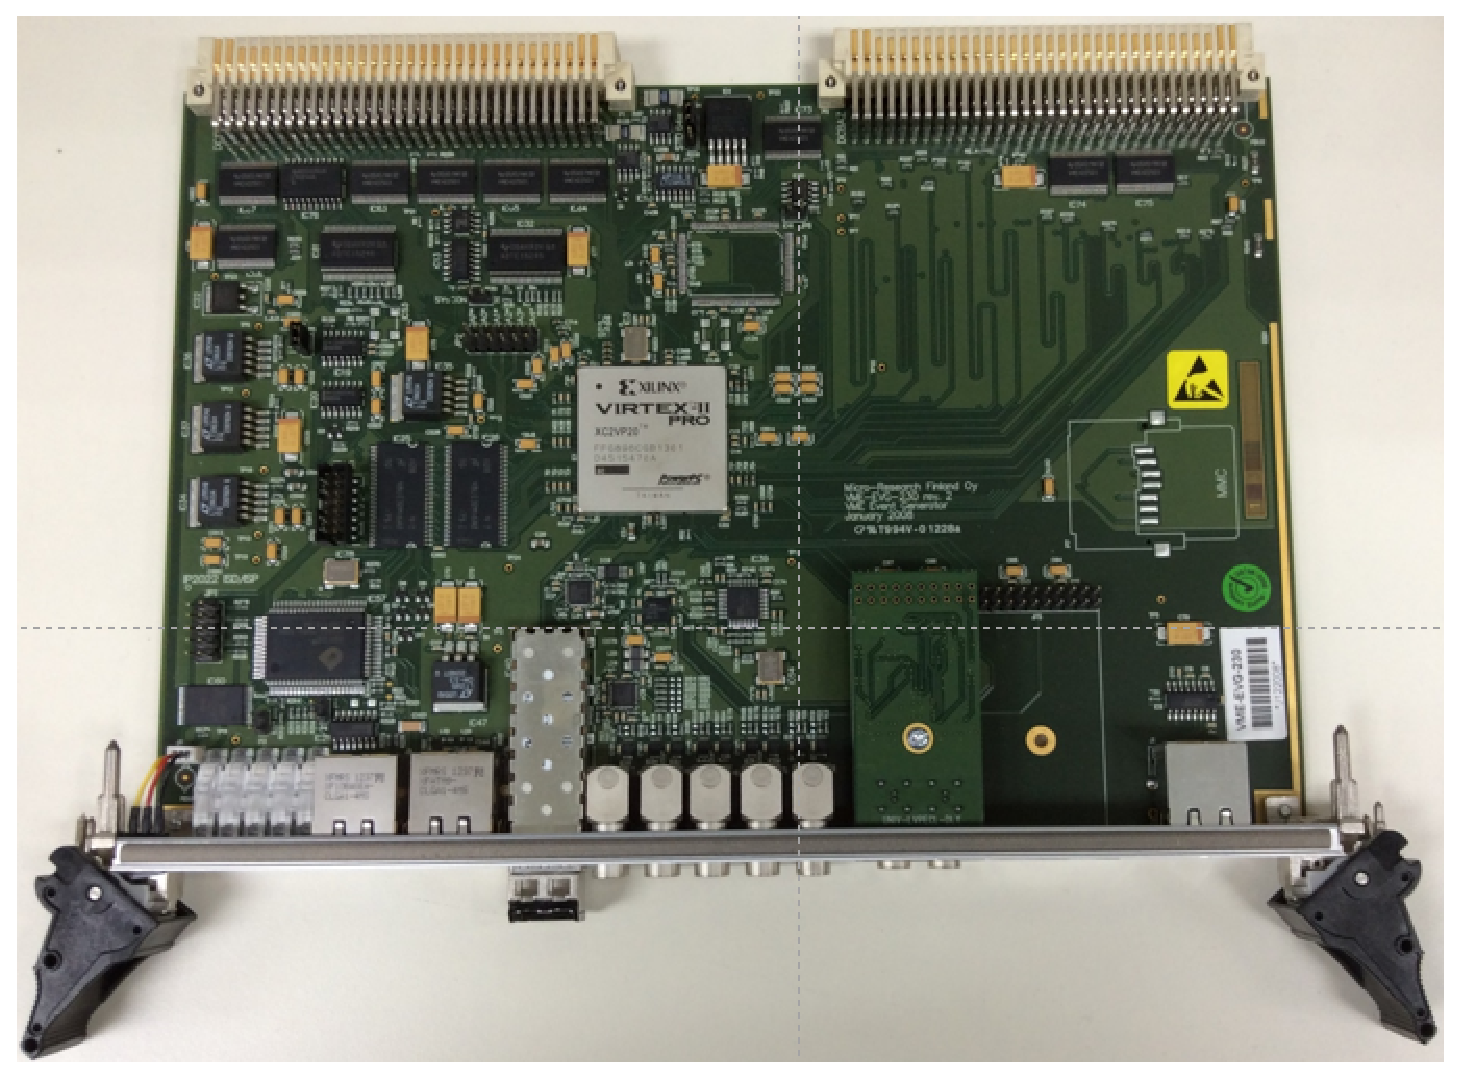
\includegraphics[width=0.8\textwidth]{./images/evg_230.eps}
	\caption{VME-EVG-230 Board}
	\label{fig:evg_230_board} 
\end{figure}

\begin{figure}[h!]
	\centering
	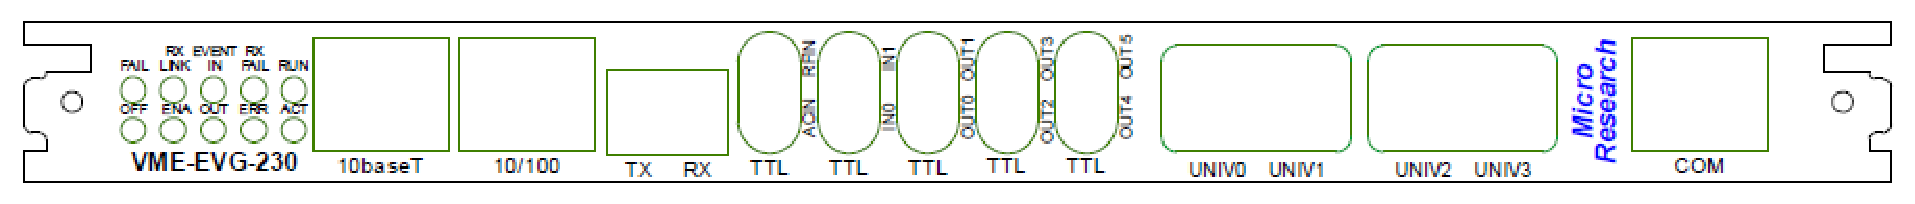
\includegraphics[width=0.8\textwidth]{./images/evg_230_front.eps}
	\caption{VME-EVG-230 Front Panel}
	\label{fig:evg_230_front} 
\end{figure}


\begin{table}[h!]
	\begin{center}
		\begin{tabular} {c|c|c|c} \hline \hline
			\cline{2-4}
			Connector/Led& Style & Level & Description \\ \hline
			FAIL  & Red Led &  & Module Failure  \\ \hline
			OFF   & Blue Led &  & Module Powered Down  \\ \hline
			RX LINK & Green Led &  & Receiver Link Signal OK  \\ \hline
			ENA & Green Led &  & Event Generator Enabled  \\ \hline	
			EVENT IN & Yellow Led &  & Incoming Event (Rx)  \\ \hline
			EVENT OUT & Yellow Led &  & Outgoing Event (Tx)  \\ \hline							
			RX FAIL & Red Led &  & Receiver Violation  \\ \hline							
			ERR & Yellow Led &  & Outgoing Event (Tx)  \\ \hline
			RUN & Green Led &  & Ubicom IP2022 Running  \\ \hline
			ACT & Yellow Led &  & Ubicom IP2022 Telnet connection active  \\ \hline
			10baseT & RJ45 & 10baseT & Ubicom 10baseT Ethernet Connection \\
			 &  &  & with link(green) and active (amber) leds \\ \hline
		 	10/100 & RJ45 &  & (reserved)  \\ \hline
			TX & LC & optical & Transmit Optical Output(TX)  \\ \hline 
			RX & LC & optical & Receiver Optical Input(RX)  \\ \hline 
			ACIN & LEMO-EPY & TTL & Trigger input  \\ \hline
			RFIN & LEMO-EPY & RF+10dBm & RF Reference Input  \\ \hline
			IN0 & LEMO-EPY & TTL & Configurable front panel input  \\ \hline
			IN1 & LEMO-EPY & TTL & Configurable front panel input  \\ \hline
			OUT0 & LEMO-EPY & TTL & Multiplexed Counter 0 Output  \\ \hline
			OUT1 & LEMO-EPY & TTL & Multiplexed Counter 1 Output  \\ \hline
			OUT2 & LEMO-EPY & TTL & Multiplexed Counter 7 Output  \\ \hline
			OUT3 & LEMO-EPY & TTL & Injection Trigger  \\ \hline
			OUT4 & LEMO-EPY & TTL & Reserved Output  \\ \hline
			OUT5 & LEMO-EPY & TTL & Reserved Output  \\ \hline
			UNIV0 & Universal I/O &  & Configurable input  \\ \hline
			UNIV1 & Universal I/O &  & Configurable input  \\ \hline
			UNIV2 & Universal I/O &  & Configurable input  \\ \hline
			UNIV3 & Universal I/O &  & Configurable input  \\ \hline
			COM   & RJ45 & RS232 & Reserved  \\ \hline
		\end{tabular}
		\caption{  Connection and status leds }
		\label{table:connection_statusled} 
	\end{center}
	\end{table} 
	
	\clearpage

\section{EVR, Event Receiver}

\begin{figure}[h!]
	\centering
	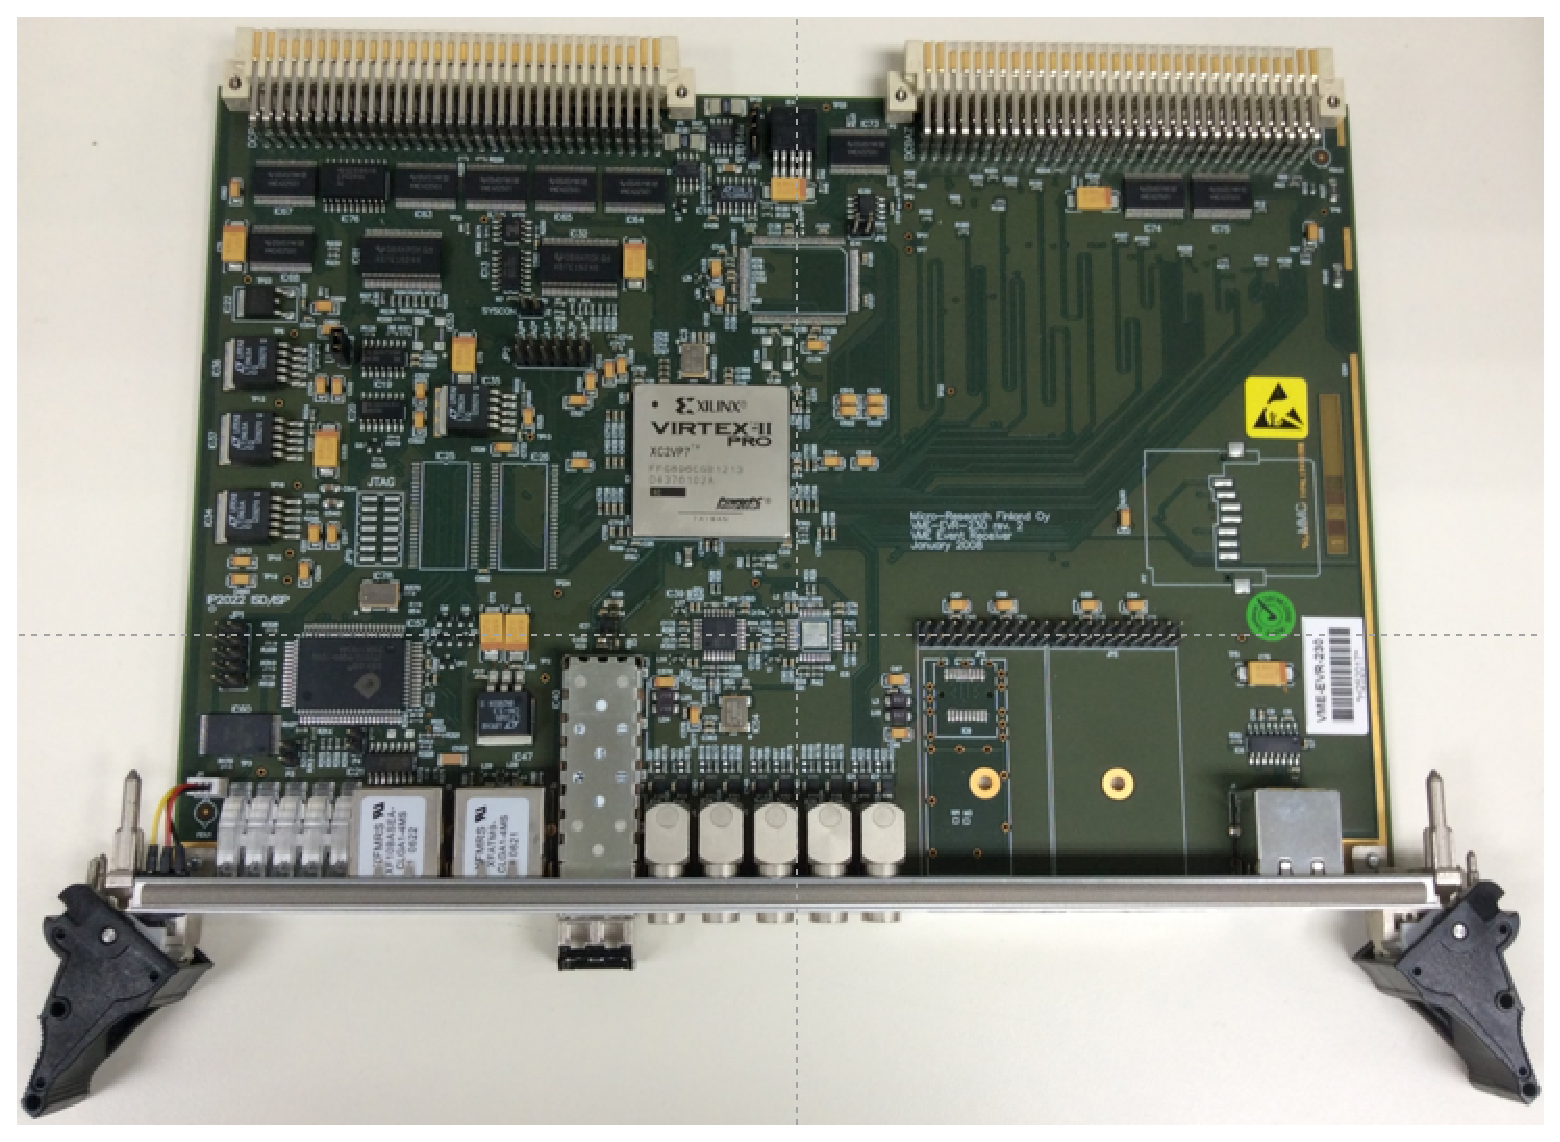
\includegraphics[width=0.8\textwidth]{./images/evr_230.eps}
	\caption{VME-EVR-230 Board}
	\label{fig:evr_230_board} 
\end{figure}

\clearpage

\section{Fanout}

\begin{figure}[h!]
	\centering
	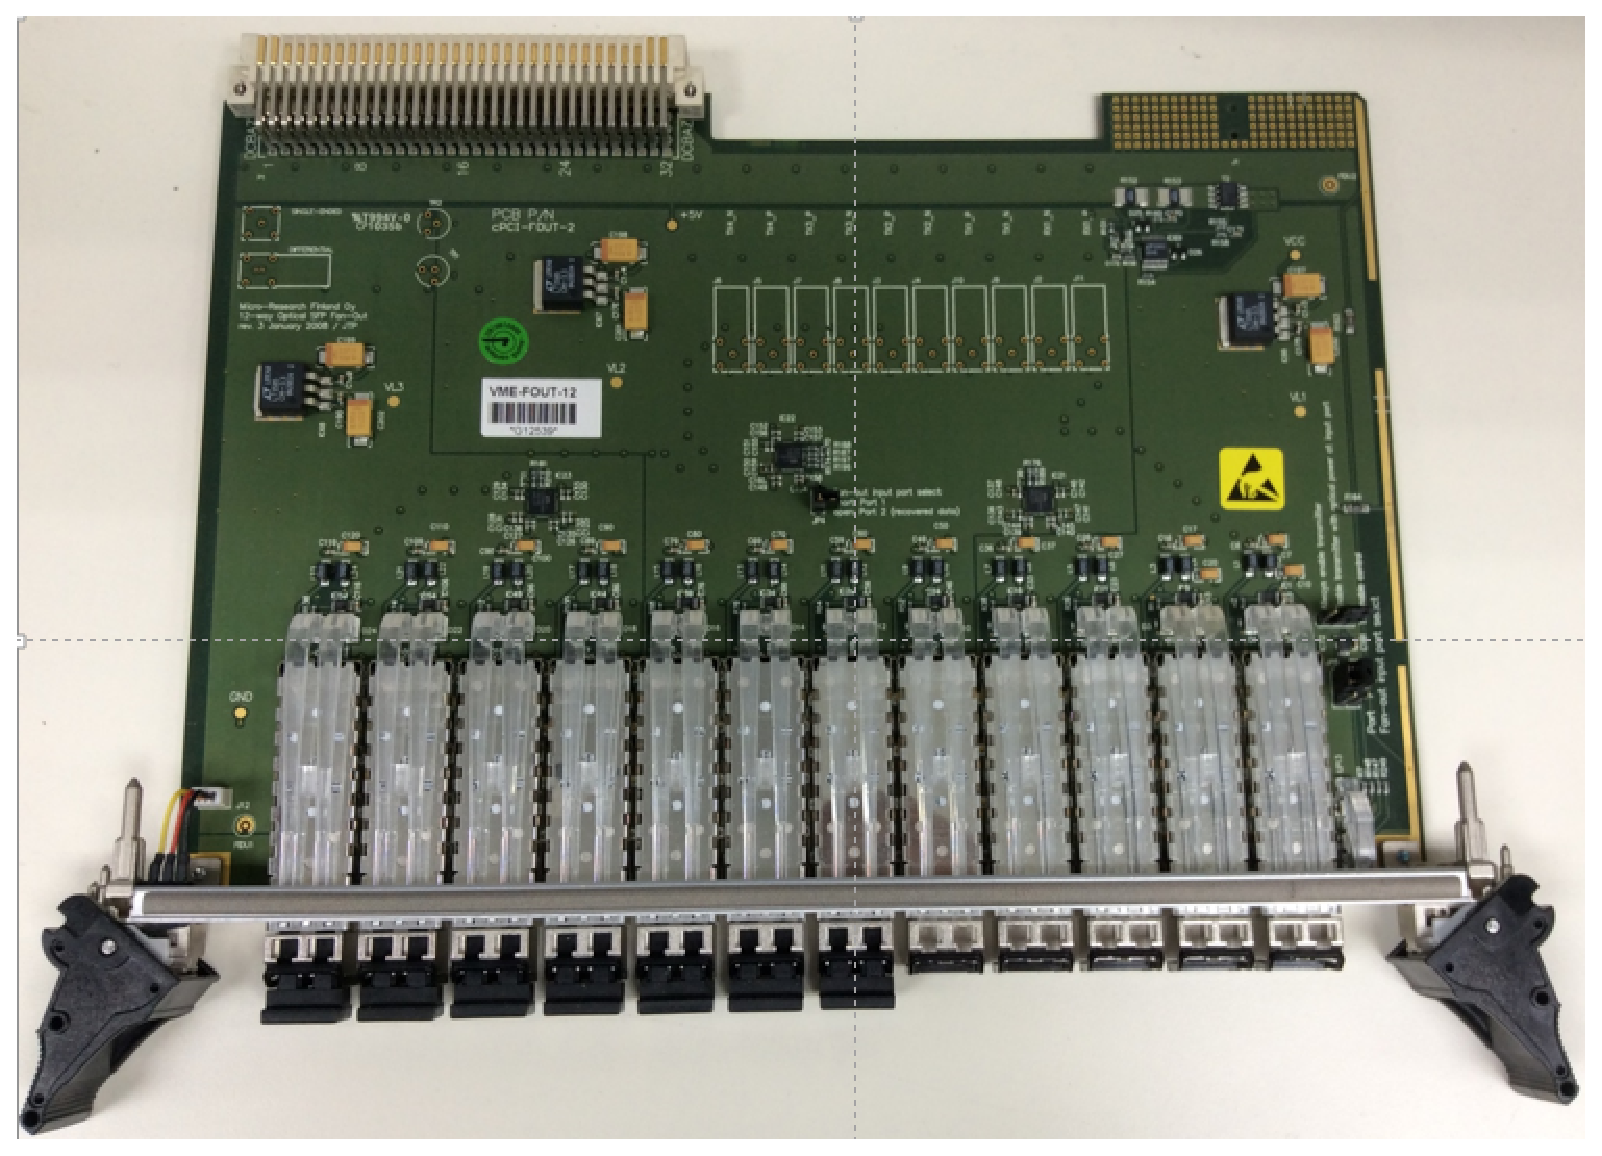
\includegraphics[width=0.8\textwidth]{./images/fanout.eps}
	\caption{VME-FANOUT Board}
	\label{fig:fanout_board} 
\end{figure}

\section{VME System}

\section{Hardware Connection}

\begin{figure}[h!]
	\centering
	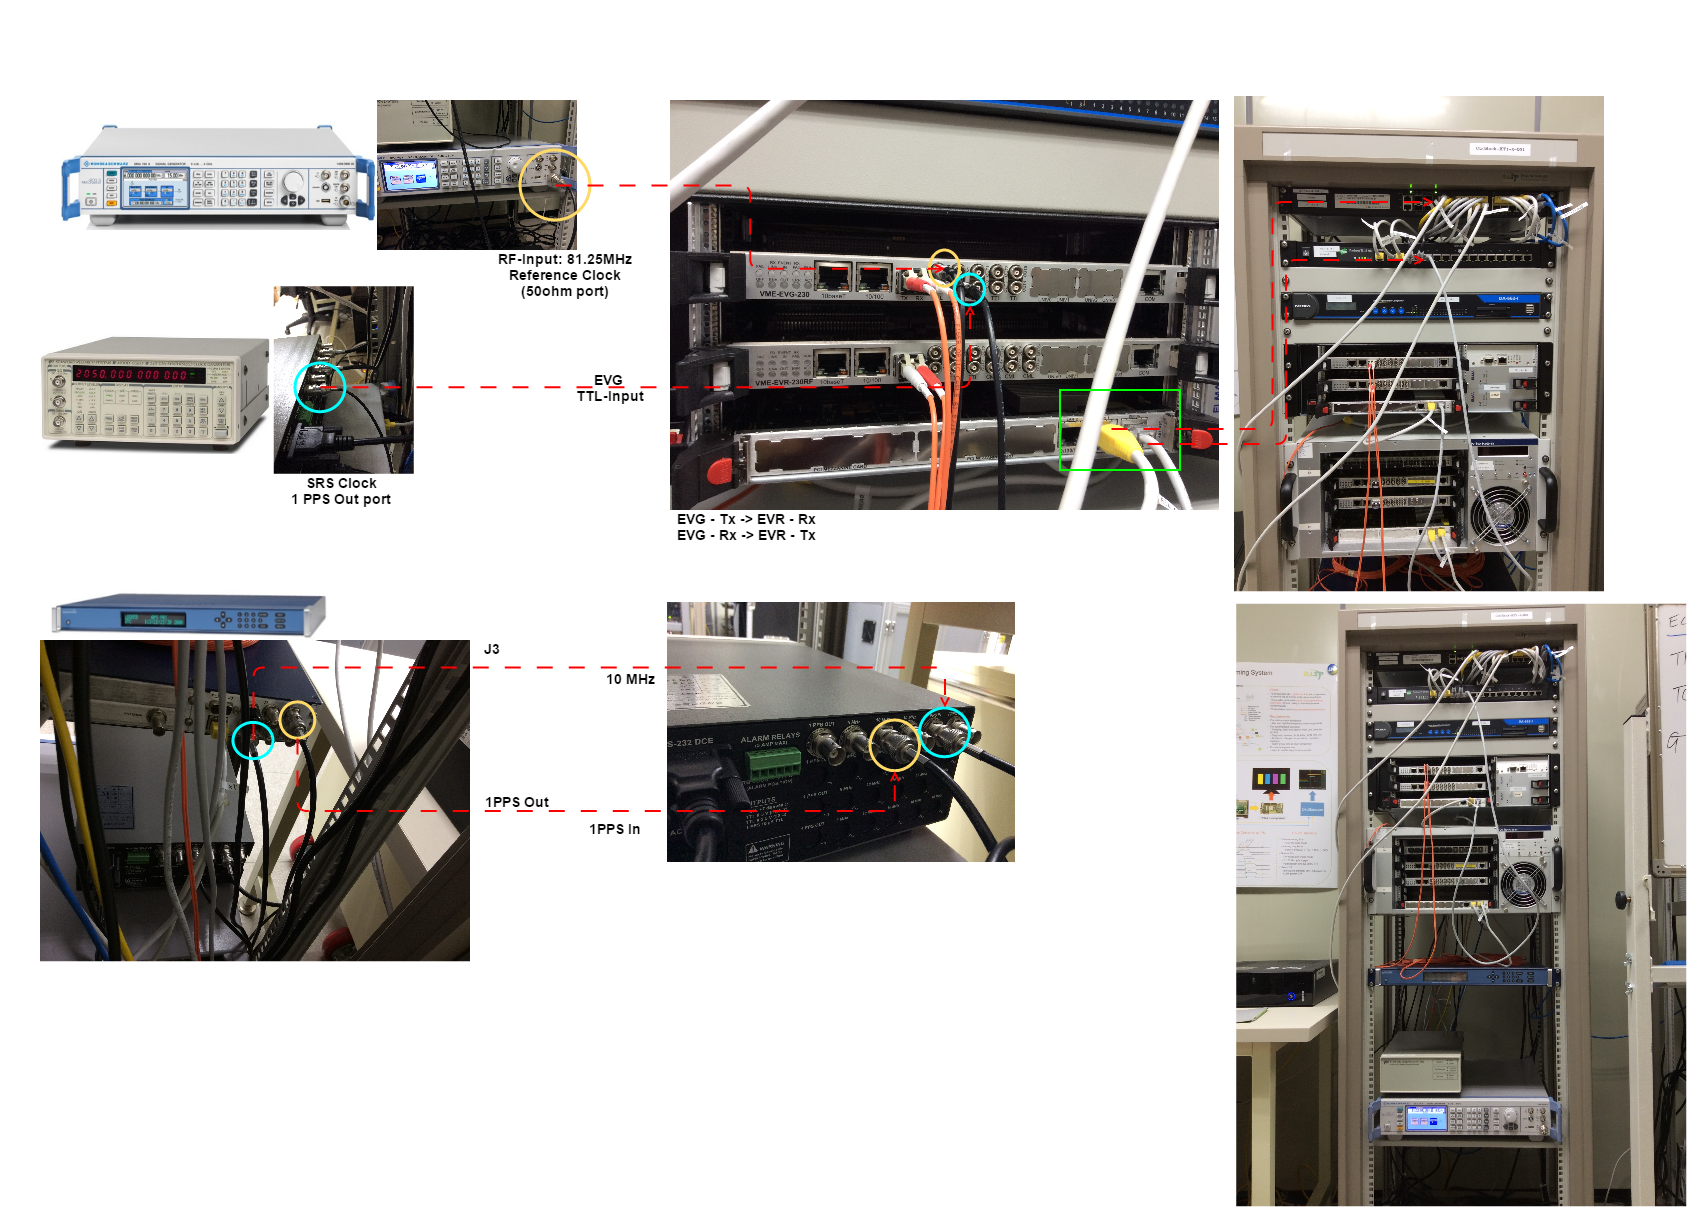
\includegraphics[width=1.1\textwidth, height=1.2\textwidth]{./images/Timing_port_connection.eps}
	\caption{Timing Port Connection}
	\label{fig:timing_port_conf} 
\end{figure}


\clearpage

\chapter{Software 구성}
\section{개발 서버 구성}
\section{운영체제 구성}

\section{MRF2IOC, EPICS IOC}

\section{VME System}


\begin{itemize}
	\item 
	\item 
\end{itemize}



\clearpage
\bibliographystyle{unsrtnat}
\bibliography{./refs}

\end{document}

